\section{Gear Train Design problem}

\subsection{Method}

\subsubsection{Continuous formulation of the gear train design}
In contrast with Task 3, which directly addressed the gear train design problem in its discrete form using stochastic optimisation, this task focuses on a deterministic local optimisation approach. To make such a method applicable, the original integer-valued design variables are relaxed to continuous variables. The gear train is therefore represented by a real-valued vector $x \in \mathbb{R}^4$, and the transmission ratio is defined as:
\begin{equation}
r(x) = \frac{x_1 x_3}{x_2 x_4}
\end{equation}
The optimisation objective is formulated as the squared deviation from a target ratio $r^*$:
\begin{equation}
f(x) = (r(x) - r^*)^2
\end{equation}
which ensures smoothness and differentiability. This continuous relaxation is not intended to be physically exact, but rather to provide a tractable framework for analysing the behaviour of gradient-based optimisation methods.

\subsubsection{Deterministic optimisation with BFGS}
The optimisation is performed using the BFGS quasi-Newton algorithm, which iteratively builds an approximation of the inverse Hessian from gradient information. Gradients are estimated numerically using finite differences, and a line search based on the Armijo condition is employed to guarantee sufficient decrease of the objective function.

Because BFGS is inherently a local method, a multi-start strategy is used, with several thousand initial points sampled within predefined bounds. The best continuous solution is then post-processed through rounding and a local integer repair step, allowing comparison with the discrete solutions obtained in Task 3.

\subsubsection{Noise robustness protocol}
To evaluate robustness, controlled additive Gaussian noise is introduced into the objective evaluations:
\begin{equation}
f_{noisy}(x) = f(x) + \sigma \mathcal{N}(0,1)
\end{equation}
where $\sigma$ denotes the noise amplitude. For each noise level, multiple independent runs are performed, and statistical indicators are computed: convergence rate, median objective value, median gradient norm at termination, integer error after repair, and median number of iterations. This protocol allows a systematic assessment of how noise affects both convergence and solution quality.

\subsection{Results}

\subsubsection{Convergence of the noise-free continuous problem}
The behaviour of BFGS on the noise-free problem is illustrated by the convergence plots of the gradient norm and the objective value.

\begin{figure}[H]
    \centering
    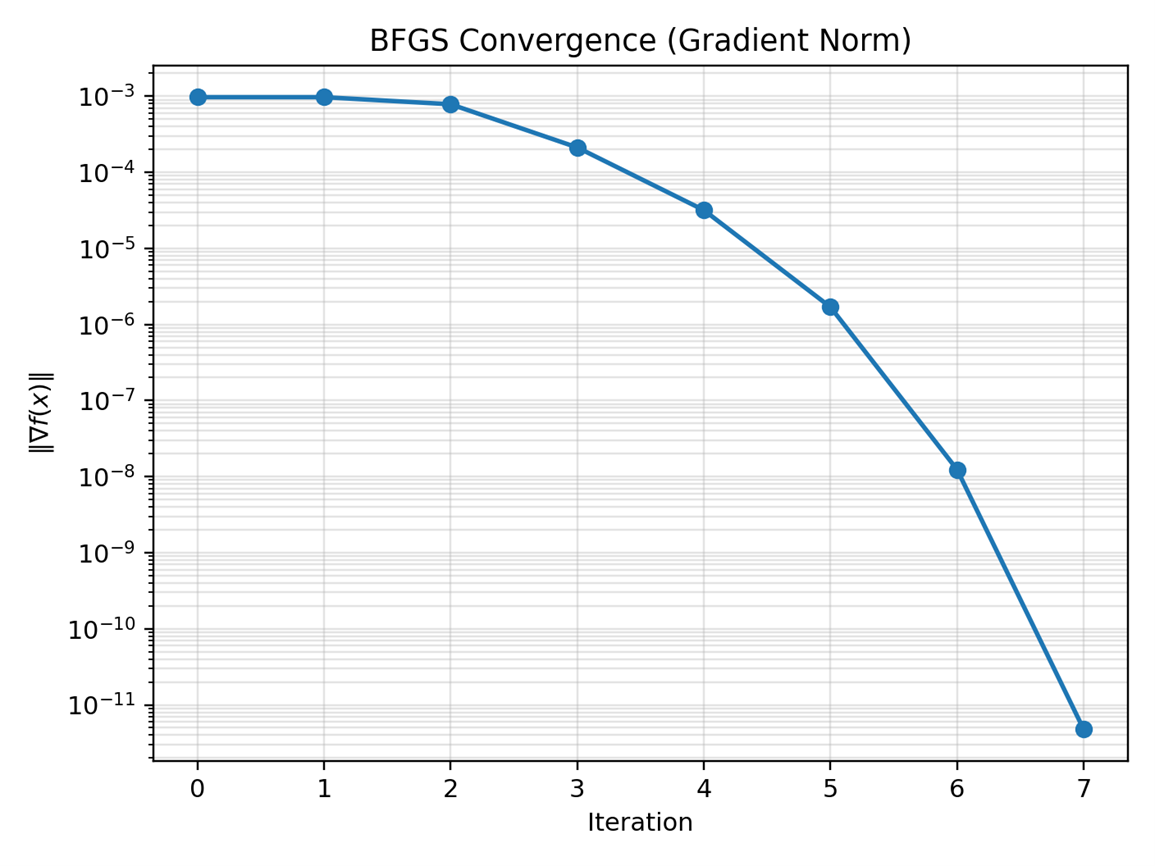
\includegraphics[width=0.8\textwidth]{Images/GearTrainDesign/BFGS Convergence(norm).png}
    \caption{BFGS Convergence (norm)}
    \label{fig:gear_bfgs_norm}
\end{figure}

As shown in Figure \ref{fig:gear_bfgs_norm}, the norm of the gradient decreases from approximately $10^{-3}$ to $10^{-11}$ in fewer than ten iterations. This represents a reduction of almost eight orders of magnitude and clearly illustrates the superlinear convergence expected from a quasi-Newton method on a smooth problem.

\begin{figure}[H]
    \centering
    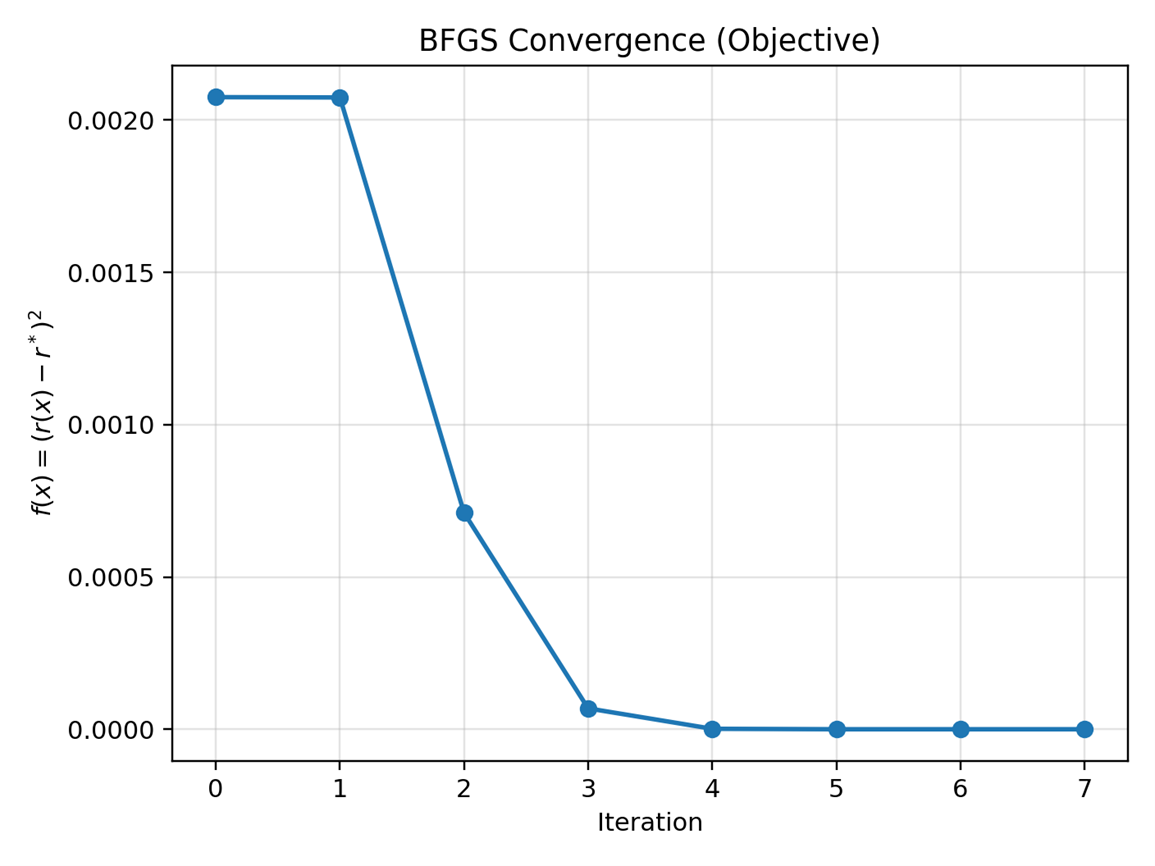
\includegraphics[width=0.8\textwidth]{Images/GearTrainDesign/BFGS Convergence(Objective).png}
    \caption{BFGS convergence (objective)}
    \label{fig:gear_bfgs_obj}
\end{figure}

A consistent picture emerges from Figure \ref{fig:gear_bfgs_obj}. After a short initial plateau, the objective value drops sharply and reaches values on the order of $10^{-20}$, corresponding to machine precision. These results confirm that, under ideal conditions, BFGS is extremely efficient for the continuous relaxation of the gear train design problem.

After rounding and integer repair, the resulting discrete solution exhibits an error of order $10^{-6}$, which is comparable to the best solutions obtained using stochastic methods, but achieved with a much smaller number of iterations.

\subsubsection{Effect of noise on convergence reliability}

\begin{figure}[H]
    \centering
    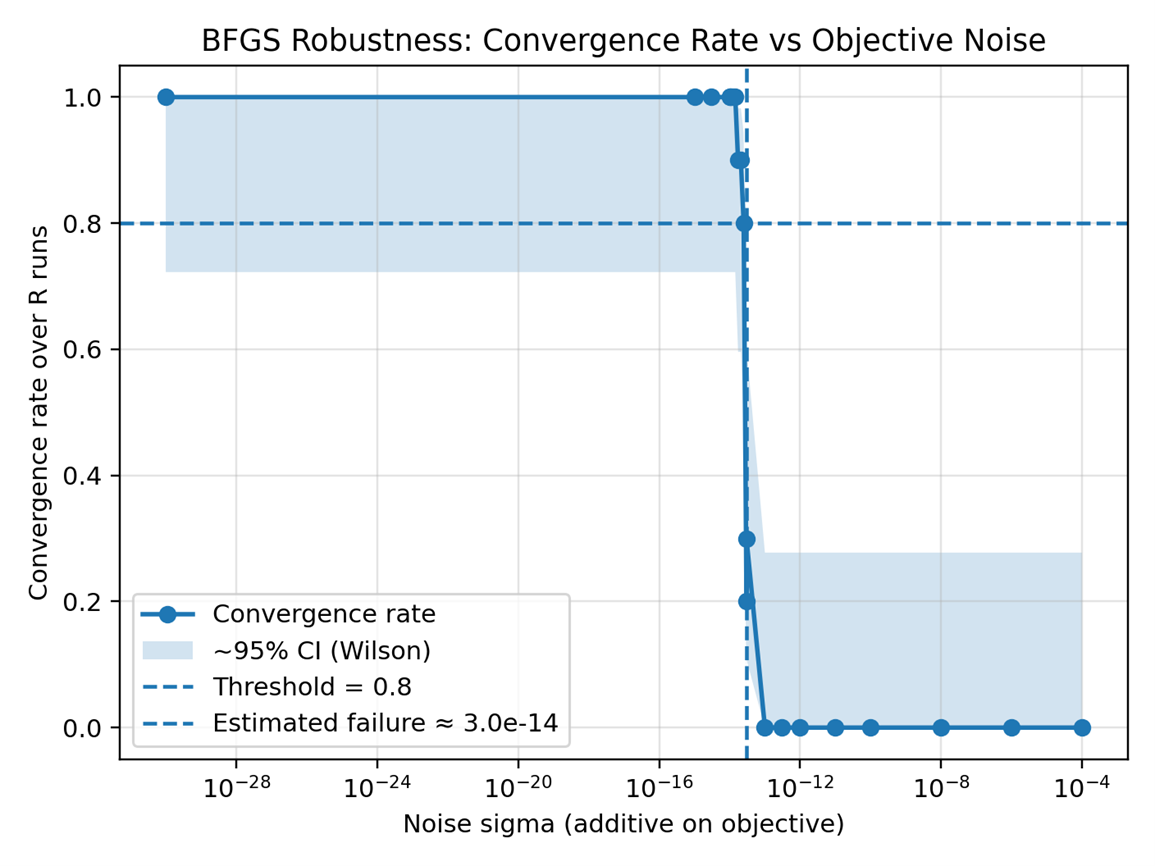
\includegraphics[width=0.8\textwidth]{Images/GearTrainDesign/BFGS robustness 1.png}
    \caption{BGFS robustness 1}
    \label{fig:gear_rob1}
\end{figure}

The impact of noise on convergence is summarised in Figure \ref{fig:gear_rob1}. For very small noise amplitudes, the convergence rate remains close to one, indicating that BFGS converges reliably in almost all runs. However, a sharp transition is observed around $\sigma \approx 3 \times 10^{-14}$, where the convergence rate drops below the imposed reliability threshold and rapidly approaches zero. This abrupt loss of convergence highlights the sensitivity of the method to perturbations in the objective.

\subsubsection{Degradation of continuous solution quality}

\begin{figure}[H]
    \centering
    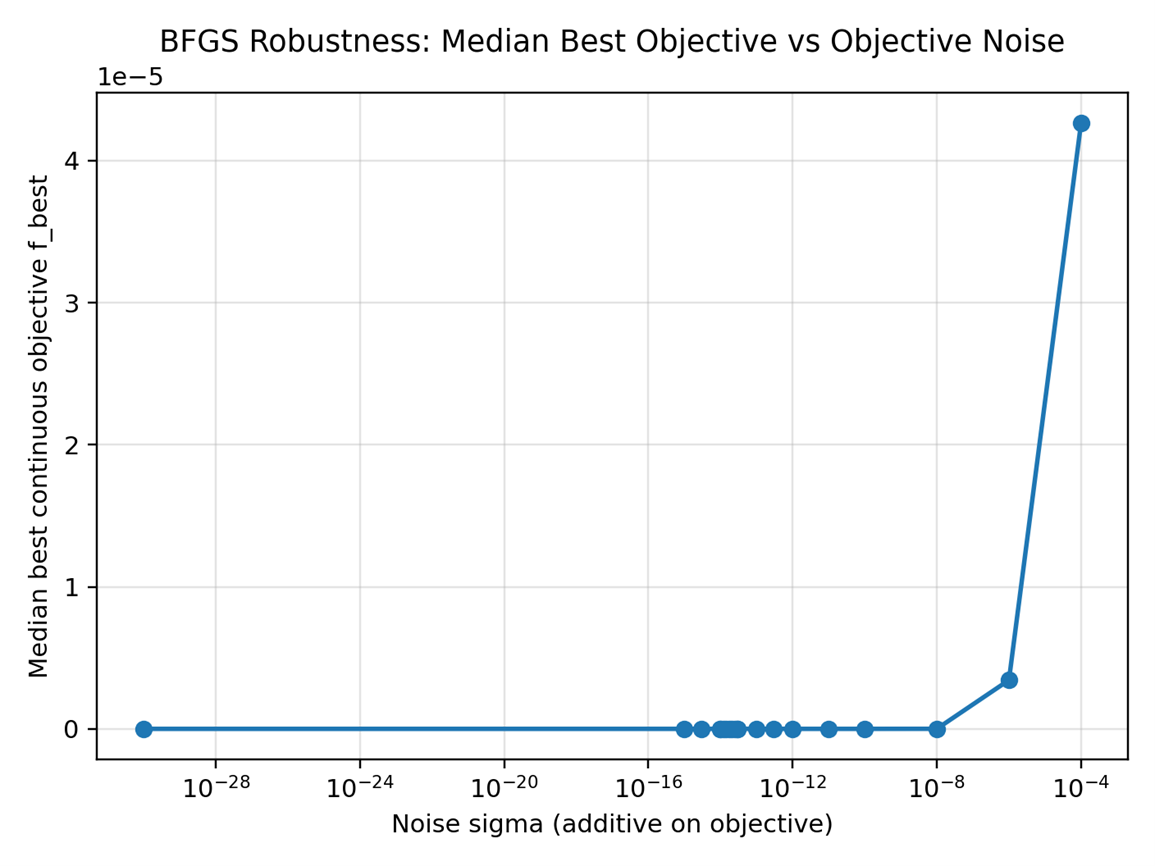
\includegraphics[width=0.8\textwidth]{Images/GearTrainDesign/BFGS robustness 2.png}
    \caption{BGFS robustness 2}
    \label{fig:gear_rob2}
\end{figure}

The deterioration of solution quality under noise is further illustrated in Figure \ref{fig:gear_rob2}. For small noise levels, the median best objective remains close to zero, indicating that accurate solutions are still found. Beyond the critical noise threshold, the objective value increases rapidly, showing that BFGS can no longer minimise the function effectively.

\begin{figure}[H]
    \centering
    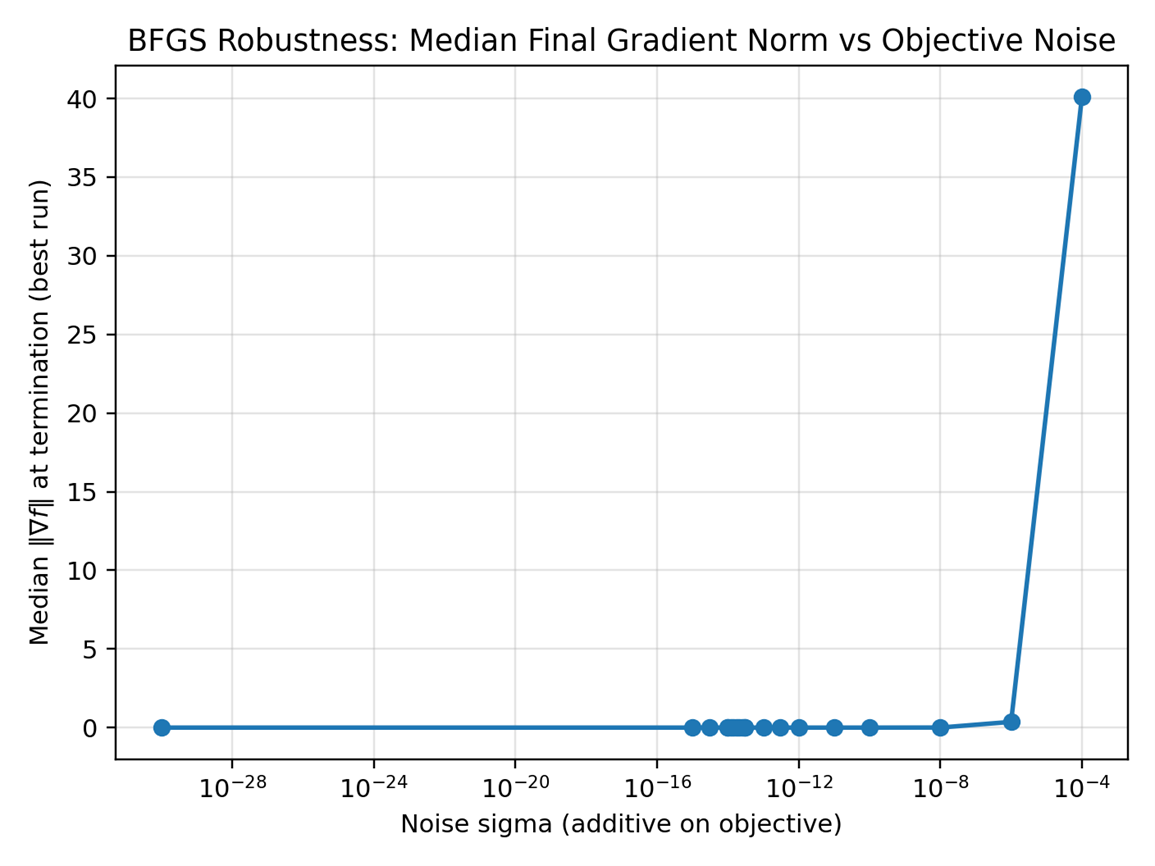
\includegraphics[width=0.8\textwidth]{Images/GearTrainDesign/BFGS robustness 3.png}
    \caption{BGFS robustness 3}
    \label{fig:gear_rob3}
\end{figure}

This behaviour is directly linked to the loss of gradient information, as confirmed by Figure \ref{fig:gear_rob3}. Once the noise exceeds the scale of the objective near the optimum, the gradient norm at termination no longer decreases and eventually grows to large values, indicating that the algorithm stops far from any stationary point.

\subsubsection{Discrete solution and computational effort}

\begin{figure}[H]
    \centering
    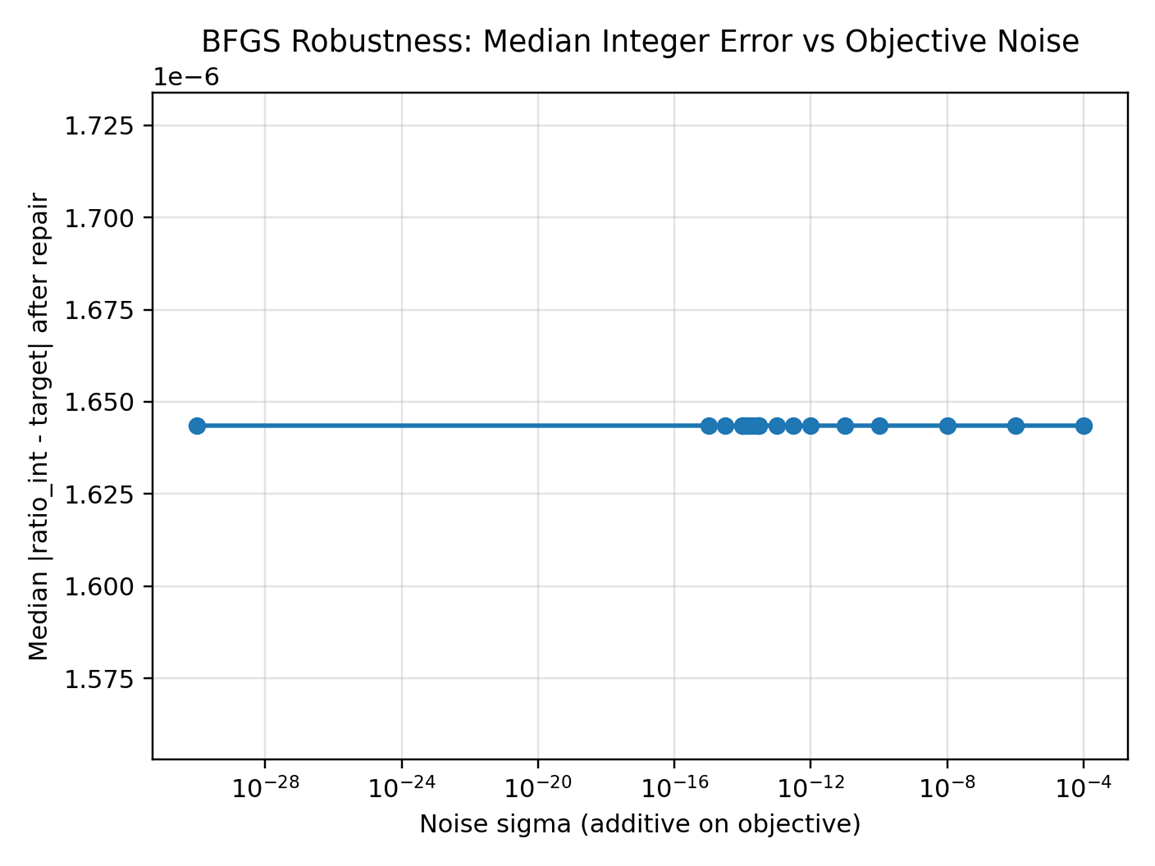
\includegraphics[width=0.8\textwidth]{Images/GearTrainDesign/BFGS robustness 4.png}
    \caption{BGFS robustness 4}
    \label{fig:gear_rob4}
\end{figure}

Interestingly, the discrete performance after rounding and repair remains remarkably stable. As shown in Figure \ref{fig:gear_rob4}, the integer error is almost unaffected by the noise level. This suggests that the multi-start strategy combined with local repair can recover the same discrete solution even when the continuous optimisation becomes unreliable.

\begin{figure}[H]
    \centering
    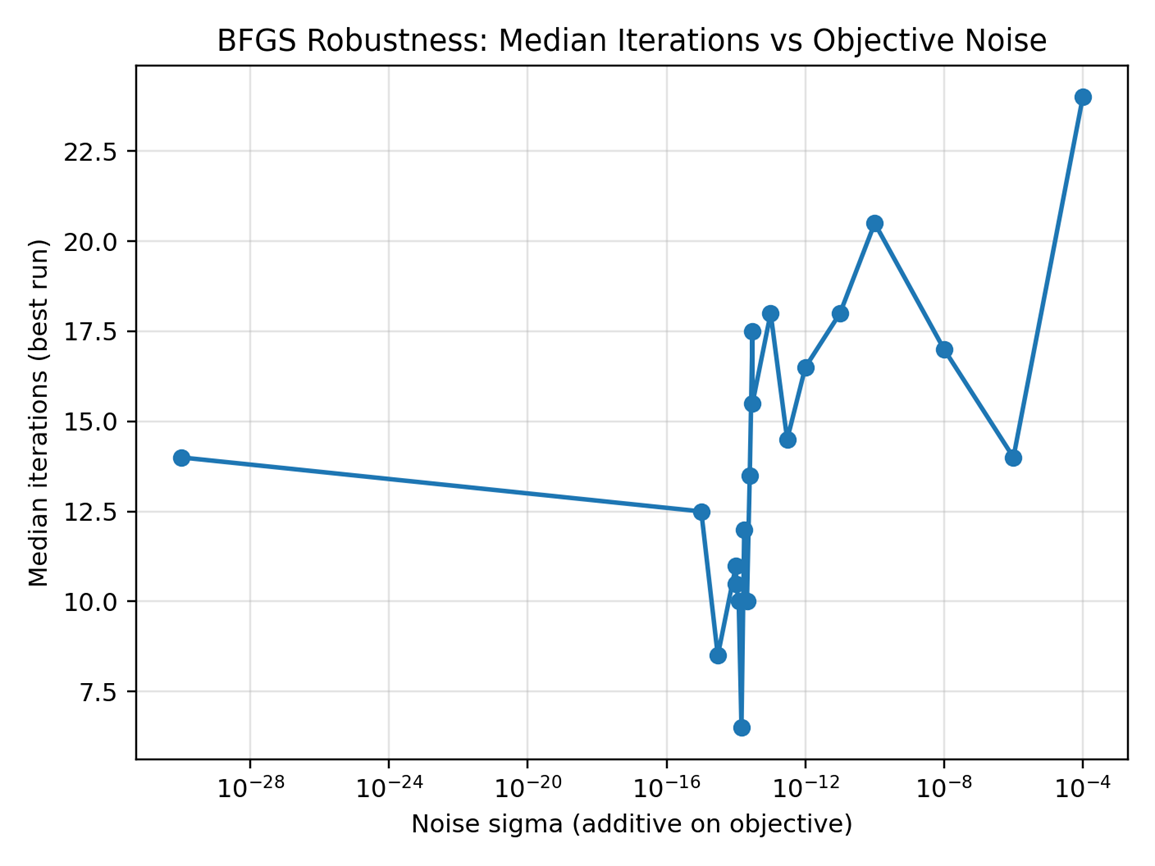
\includegraphics[width=0.8\textwidth]{Images/GearTrainDesign/BFGS robustness 5.png}
    \caption{BGFS robustness 5}
    \label{fig:gear_rob5}
\end{figure}

Finally, Figure \ref{fig:gear_rob5} shows that the number of iterations increases and becomes more irregular as noise grows. This indicates a loss of efficiency and predictability before the complete failure of convergence.

\subsubsection{Supplementary analysis of noise effect}
The following values were obtained by displaying these variables at different stages of the program.

\begin{table}[H]
    \centering
    \resizebox{\textwidth}{!}{
    \begin{tabular}{|l|l|l|l|l|l|l|}
    \hline
    Regime & Noise $\sigma$ & Convergence rate & Median $f_{best}$ & Median $||\nabla f||$ & Median integer error & Median iterations \\ \hline
    Low noise & $1.0\times 10^{-15}$ & 1.00 & $-2.8\times 10^{-16}$ & $5.1\times 10^{-10}$ & $2.0\times 10^{-6}$ & 12.5 \\ \hline
    Transition & $3.0\times 10^{-14}$ & 0.20 & $-1.9\times 10^{-14}$ & $1.3\times 10^{-8}$ & $2.0\times 10^{-6}$ & 17.5 \\ \hline
    High noise & $1.0\times 10^{-4}$ & 0.00 & $4.3\times 10^{-5}$ & $4.0\times 10^{-16}$ & $2.0\times 10^{-6}$ & 24.0 \\ \hline
    \end{tabular}
    }
    \caption{Regime comparison}
    \label{tab:gear_regime}
\end{table}

In the low-noise regime, BFGS behaves as expected for a smooth continuous problem: convergence is reliable, the final gradient norm is extremely small, and the objective value reaches machine-level precision within a limited number of iterations. This confirms both the efficiency and numerical stability of the method under ideal conditions.

At the transition noise level, convergence reliability deteriorates sharply even though objective values and gradient norms remain relatively small in absolute terms. This indicates that loss of reliability precedes complete numerical divergence, as the algorithm struggles to maintain consistent descent directions and line-search acceptance.

In the high-noise regime, BFGS fails as a local optimiser: gradient norms grow by several orders of magnitude, and the objective value degrades significantly. However, the discrete solution obtained after rounding and repair remains essentially unchanged, demonstrating that the post-processing step is largely decoupled from the behaviour of the continuous solver under noise.

\subsection{Discussion}
The results demonstrate that BFGS is exceptionally effective for the noise-free continuous relaxation of the gear train design problem. Its rapid convergence and high precision make it a powerful tool for local optimisation and for understanding the structure of the objective function.

However, the robustness analysis reveals a fundamental limitation. Near the optimum, the objective value is of order $10^{-20}$, meaning that even extremely small absolute noise levels dominate the signal. As a result, finite-difference gradients and line-search conditions become unreliable, leading to the abrupt convergence breakdown observed around $\sigma \approx 3 \times 10^{-14}$. This behaviour is clearly visible in the convergence rate and gradient norm figures and reflects the strong assumptions underlying deterministic gradient-based methods.

The stability of the integer error despite the loss of continuous convergence highlights the role of post-processing and global sampling. While BFGS itself fails under noise, the surrounding strategy can still recover acceptable discrete solutions, masking the underlying loss of theoretical validity.

When compared to the stochastic approaches used in Task 3, these findings clarify the complementary nature of the methods that allow us to choose between efficiency and precision or robustness. For practical gear train design problems, which are discrete and subject to modelling uncertainty, this strongly supports the use of global stochastic optimisation as the primary approach, with deterministic local methods serving as refinement tools rather than standalone solvers.
